%%%%%%%%%%%%%%%%%%%%%%%%%%%%%%%%%%%%%%%%%
% Masters/Doctoral Thesis 
% LaTeX Template
% Version 2.5 (27/8/17)
%
% This template was downloaded from:
% http://www.LaTeXTemplates.com
%
% Version 2.x major modifications by:
% Vel (vel@latextemplates.com)
%
% This template is based on a template by:
% Steve Gunn (http://users.ecs.soton.ac.uk/srg/softwaretools/document/templates/)
% Sunil Patel (http://www.sunilpatel.co.uk/thesis-template/)
%
% Template license:
% CC BY-NC-SA 3.0 (http://creativecommons.org/licenses/by-nc-sa/3.0/)
%
%%%%%%%%%%%%%%%%%%%%%%%%%%%%%%%%%%%%%%%%%

%----------------------------------------------------------------------------------------
%	PACKAGES AND OTHER DOCUMENT CONFIGURATIONS
%----------------------------------------------------------------------------------------

\documentclass[
11pt, % The default document font size, options: 10pt, 11pt, 12pt
oneside, % Two side (alternating margins) for binding by default, uncomment to switch to one side
english, % ngerman for German
singlespacing, % Single line spacing, alternatives: onehalfspacing or doublespacing
%draft, % Uncomment to enable draft mode (no pictures, no links, overfull hboxes indicated)
%nolistspacing, % If the document is onehalfspacing or doublespacing, uncomment this to set spacing in lists to single
%liststotoc, % Uncomment to add the list of figures/tables/etc to the table of contents
%toctotoc, % Uncomment to add the main table of contents to the table of contents
%parskip, % Uncomment to add space between paragraphs
%nohyperref, % Uncomment to not load the hyperref package
headsepline, % Uncomment to get a line under the header
%chapterinoneline, % Uncomment to place the chapter title next to the number on one line
%consistentlayout, % Uncomment to change the layout of the declaration, abstract and acknowledgements pages to match the default layout
table,
]{MastersDoctoralThesis} % The class file specifying the document structure

\usepackage[utf8]{inputenc} % Required for inputting international characters
\usepackage[T1]{fontenc} % Output font encoding for international characters

\usepackage{mathpazo} % Use the Palatino font by default
\usepackage{float}

\usepackage[backend=bibtex,style=authoryear,natbib=true,doi=false]{biblatex} % Use the bibtex backend with the authoryear citation style (which resembles APA)

\addbibresource{references.bib} % The filename of the bibliography

\usepackage[autostyle=true]{csquotes} % Required to generate language-dependent quotes in the bibliography
\usepackage{eurosym}

\usepackage{amsmath,amsfonts,amssymb}
\usepackage[linesnumbered,ruled]{algorithm2e}
\SetKwInput{KwInput}{Input}
\SetKwInput{KwOutput}{Output} 

\usepackage{subcaption}

%----------------------------------------------------------------------------------------
%	MARGIN SETTINGS
%----------------------------------------------------------------------------------------

\geometry{
	paper=a4paper, % Change to letterpaper for US letter
	inner=2.5cm, % Inner margin
	outer=3.8cm, % Outer margin
	bindingoffset=.5cm, % Binding offset
	top=1.5cm, % Top margin
	bottom=1.5cm, % Bottom margin
	%showframe, % Uncomment to show how the type block is set on the page
}

%----------------------------------------------------------------------------------------
%	THESIS INFORMATION
%----------------------------------------------------------------------------------------

\thesistitle{Analysis of the SVM-RFE algorithm for feature selection} % Your thesis title, this is used in the title and abstract, print it elsewhere with \ttitle
\supervisor{Luis A. \textsc{Belanche}} % Your supervisor's name, this is used in the title page, print it elsewhere with \supname
\examiner{} % Your examiner's name, this is not currently used anywhere in the template, print it elsewhere with \examname
\degree{Bachelor Degree in Informatics Engineering} % Your degree name, this is used in the title page and abstract, print it elsewhere with \degreename
\author{Robert \textsc{Planas}} % Your name, this is used in the title page and abstract, print it elsewhere with \authorname
\addresses{} % Your address, this is not currently used anywhere in the template, print it elsewhere with \addressname

\subject{Computing} % Your subject area, this is not currently used anywhere in the template, print it elsewhere with \subjectname
\keywords{} % Keywords for your thesis, this is not currently used anywhere in the template, print it elsewhere with \keywordnames
\university{\href{http://www.upc.edu}{Universitat Politècnica de Catalunya}} % Your university's name and URL, this is used in the title page and abstract, print it elsewhere with \univname
\department{ \_ } % Your department's name and URL, this is used in the title page and abstract, print it elsewhere with \deptname
\group{ \_ } % Your research group's name and URL, this is used in the title page, print it elsewhere with \groupname
\faculty{Facultat d'informàtica de Barcelona} % Your faculty's name and URL, this is used in the title page and abstract, print it elsewhere with \facname

\AtBeginDocument{
\hypersetup{pdftitle=\ttitle} % Set the PDF's title to your title
\hypersetup{pdfauthor=\authorname} % Set the PDF's author to your name
\hypersetup{pdfkeywords=\keywordnames} % Set the PDF's keywords to your keywords
}

\begin{document}

\frontmatter % Use roman page numbering style (i, ii, iii, iv...) for the pre-content pages

\pagestyle{plain} % Default to the plain heading style until the thesis style is called for the body content

%----------------------------------------------------------------------------------------
%	TITLE PAGE
%----------------------------------------------------------------------------------------

\begin{titlepage}
\begin{center}

\vspace*{.06\textheight}
{\scshape\LARGE \univname\par}\vspace{0.5cm} % University name
\textsc{\Large \facname}\\[1.5cm] % Facultry name
\Large{\emph{Draft}}\\[0.5cm] % Thesis type

\HRule \\[0.4cm] % Horizontal line
{\huge \bfseries \ttitle\par}\vspace{0.4cm} % Thesis title
\HRule \\[1.5cm] % Horizontal line
 
\begin{minipage}[t]{0.4\textwidth}
\begin{flushleft} \large
\emph{Author:}\\
\href{http://www.hubbit86.com}{\authorname} % Author name - remove the \href bracket to remove the link
\end{flushleft}
\end{minipage}
\begin{minipage}[t]{0.4\textwidth}
\begin{flushright} \large
\emph{Director:} \\
\href{https://www.cs.upc.edu/~belanche/}{\supname} % Supervisor name - remove the \href bracket to remove the link  
\end{flushright}
\end{minipage}\\[4cm]

\vfill

\large \degreename\\ % Speciality name
\large Specialization:  Computing\\[0.5cm] % Speciality name

\vfill

% \large \textit{A thesis submitted in fulfillment of the requirements\\ for the degree of \degreename}\\[0.3cm] % University requirement text
% \textit{in the}\\[0.4cm]
% \groupname\\\deptname\\[2cm] % Research group name and department name

\includegraphics{img/logo.pdf} % University/department logo - uncomment to place it

\vfill

{\large \today}\\[4cm] % Date

\vfill
\end{center}
\end{titlepage}



%----------------------------------------------------------------------------------------
%	THESIS CONTENT - CHAPTERS
%----------------------------------------------------------------------------------------

\newcommand{\tabhead}[1]{\textbf{#1}}
\newcommand{\VS}{\vspace{6pt}}
\newcommand{\vt}[1]{\vec{#1}}
\newcommand{\st}{\ |\ }
\newcommand{\vb}[1]{\mathbf{#1}}
\newcommand{\T}{\text{T}}

\mainmatter % Begin numeric (1,2,3...) page numbering

\pagestyle{thesis} % Return the page headers back to the "thesis" style
\tableofcontents
% Chapter 1

\chapter{Introduction} % Main chapter title

\label{Chapter1} % For referencing the chapter elsewhere, use \ref{Chapter1} 

%----------------------------------------------------------------------------------------

This bachelor thesis at the Computer Engineering Degree, specialization in Com\-puting, has been done in the Facultat d’Informàtica de Barcelona of the Universitat Politècnica de Catalunya (UPC) and directed by Luis Antonio Belanche Muñoz, PhD. in Computer Science.

\section{Context}
\label{sec:context}

In statistics, machine learning, data-mining, and other related disciplines, it is often the case that there are redundant or irrelevant data in a dataset\footnote{A table with rows / records / observations and columns / variables / features / dimensions / predictors / attributes.}. Indeed, before we can start working with the data, some form of data analysis and cleaning is required. Data cleaning may include removing duplicated rows or rows with missing values, removing observations that are clearly outliers, removing irrelevant variables (e.g. name, surname, email address), etc.

With the new era of Big Data, datasets have increased in size, both in number of observations and in dimensions. Applying classical data-mining and machine learning algorithms to these high-dimensional data raise multiple issues collectively known as “the curse of dimensionality”. One such issue is the elevated, usually intractable, cost and memory requirements derived from the non-linear (on number of dimensions and observations) complexities of the algorithms. Another issue has to do with data in a high-dimensional space becoming sparse and negatively af\-fect\-ing the performance of algorithms designed to work in a low-dimensional space. And finally, a third issue is that with a high number of dimensions the algorithms tend to overfit, that is, they don't generalize enough and end up producing models that perform worse with real data than their predicted performance with the training data. (\cite{li_feature_2017})

Simple manual data cleaning is not enough to achieve satisfactory amounts of dimensionality reduction. In this case we can use automatic techniques. We can classify such techniques in two categories: feature extraction and feature selection.

\subsection{Feature extraction}

Feature extraction techniques transform the original high-dimensional space into a new low-dimensional space by extracting or deriving information from the original features. The premise is to compress the data in order to pack the same information at the expense of model explainability\footnote{The ability to explain why certain predictions are made. Also, interpretability.}. Continuing with our data compression analogy, virtually all feature extraction techniques perform lossy com\-pres\-sion. That is, some information is lost which makes the process irreversible. 

Some well known feature extraction algorithms include Principal Component Analysis (PCA) (\cite{scholkopf_kernel_1997}) and auto-encoders (\cite{vincent_extracting_2008}), the first being a transformation over the feature-space and the second a neuronal network. PCA may be extended with a kernel method in order to make non-linear transformations. Similarly, we will also use non-linear kernels in some of our extensions.

\subsection{Feature selection}
\label{sec:ch1.feature_selection}

In contrast, feature selection only selects a subset of the existing features, ideally the most relevant or useful. This may imply a greater loss of information compared to feature extraction, but it doesn't reduce explainability. Some problems require feature selection explicitly. In domains such as genetic analysis and text mining, feature selection is not necessarily used to build predictors. For example in micro\-array analysis feature selection is used to identify genes (i.e. features) that dis\-criminate between healthy and sick patients. 

Note that the number of possible selections of all sizes is $2^m$. This is the same as the amount of subsets of a set with size $m$, where $m$ is the amount of total features. The number of possible selections for some feature subset size $k$, is then ${m \choose k} = \frac{m!}{k!(m - k)!}$. This makes the optimal feature selection via exhaustive search intractable. Instead, we use methods that do not require an exhaustive search, such as a greedy algorithm, at the expense of not being able to guarantee an optimal solution.

Feature selection methods may be classified by how they are constructed in three categories:

\begin{itemize}
    \item \textbf{Filters:} A \emph{feature ranking criterion} is used to sort the features in order of rel\-e\-vance, then select the $k$-most relevant.
    \item \textbf{Wrappers:} They use a learning machine (treated as a black box) to train and validate the dataset with different subsets of variables. They rank the subsets based on the performance (score) of the model. A wide range of learning machines and search strategies can be used. Within the greedy strategies we find \emph{forward selection} and \emph{backward elimination}.
    \item \textbf{Embedded:} Like wrapper methods but more efficient. They use information from the model itself at training time to make feature selection. Because they don't use the score, they can also skip testing the model.
\end{itemize}

In both wrapper and embedded methods greedy strategies can be used. \textbf{SVM-RFE} is a feature selection algorithm, of the embedded class, that uses Support Vector Machines (SVM) and a greedy strategy called Recursive Feature Elimination (RFE). This algorithm is an instance of backward elimination. It starts with a set of all features and eliminates the less relevant each iteration. Within each iteration SVM-RFE behaves like a filter method and uses a feature ranking criterion to decide which feature to eliminate. SVM-RFE takes advantage of the fact that, for linear SVM, the ranking criterion is to take the variable with the smallest absolute weight in each iteration. Where the weights are the co\-ef\-fi\-cients of the hyperplane resulting from the SVM training.  (\cite{guyon_introduction_2003})

%----------------------------------------------------------------------------------------

\section{State of the art}

The SVM-RFE algorithm was first proposed in a paper on the topic of cancer class\-ification (\cite{guyon_gene_2002}). This paper uses the SVM-RFE algorithm to identify highly discriminant genes, encoded as features, that have plausible relevance to cancer diagnosis. Since then, SVM-RFE has remained a popular technique for gene selection and the original paper cited more than four thousand times.

The paper already proposes some natural extensions to the al\-go\-rithm, such as eliminating multiple features each iteration based on the ranking and a \emph{step} constant. Further research has been on improving and extending different parts of the al\-go\-rithm. These include the use of a Gaussian kernel (\cite{xue_nonlinear_2018}), using multiple SVM in the same iteration (\cite{wang_classification_2011}) or simply trying to find a better ranking criterion (\cite{mundra_svm-rfe_2007}).

%----------------------------------------------------------------------------------------

\section{Project goals}
\label{sec:ch1.objective}

The main objective of this project is to research possible extensions and im\-prove\-ments that try to optimize the SVM-RFE algorithm. Optimizations may be in the form of improved performance or a reduction in time utilization. We do not propose here any optimizations that may affect space complexity. As such, we also skip the space complexity analysis for the whole project. We've classified the possible extensions as follows.

\subsubsection*{Main extensions}

These focus on improving the performance of the selection of features.

\begin{itemize}
    \item \textbf{Non-linear kernel:} Use a more general ranking criterion and apply it to handle SVM with arbitrary kernels.
    \item \textbf{Multi-class criteria:} Find a ranking criterion that can handle multiple weight vectors in a useful way.
\end{itemize}

\subsubsection*{Secondary extensions}

Focus on reducing the computational cost.

\begin{itemize}
    \item \textbf{Internal sampling:} Use a different subset of the observations on each iteration.
    \item \textbf{Dynamic step:} Instead of using a constant value in each iteration, calculate it dynamically.
    \item \textbf{Stop condition:} Determine the amount of features that are relevant (SVM-RFE only provides a ranking) in an effective and inexpensive manner.
\end{itemize}

\subsubsection*{Combination of various extensions}

\begin{itemize}
    \item \textbf{Combo:} Mix \emph{internal sampling}, \emph{dynamic step} and \emph{non-linear Kernels} into a single implementation.
\end{itemize}

\subsection{Goals break down}

To accomplish these goals, the project has been sub\-divided in two parts, each having specific tasks for each extension:

\subsubsection*{Algorithmic Part}

\begin{itemize}
    \item Do research in SVM-RFE and in the extensions that will be tackled in the project.
    \item {
        For each extension:
        \begin{itemize}
            \item Design the algorithm and write its formalization in pseudocode.
            \item Define the expected advantages or disadvantages of this extension over the base SVM-RFE.
            \item Compute the time complexity.
        \end{itemize}
    }
\end{itemize}

\subsubsection*{Practical Part}

\begin{itemize}
    \item Program the base SVM-RFE algorithm and the extensions.
    \item {
        For each extension:
        \begin{itemize}
            \item Analyze its behavior for artificial data sets.
            \item Analyze its behavior for real-world data sets.
        \end{itemize}
    }
    \item Compare the results obtained with the ones expected.
    \item Combine multiple extensions to further improve the algorithm.
    \item Draw conclusions about all the results obtained in the project.
\end{itemize}

%----------------------------------------------------------------------------------------

\subsection{Stakeholders}

This project is intended to be of use for many involved parties. The most directly involved group, is the tutor and the researcher. Luis Antonio Belanche Muñoz is the tutor of this project. Robert Planas Jimenez would be the researcher. Feature selection algorithms is one of the areas of research of the tutor, and he has wanted to explore extensions to the SVM-RFE algorithm. He will lead and guide the researcher for the correct development of the project. The researcher is responsible for planning, developing and documenting the project, as well as experimenting, analyzing and drawing conclusions.

The other group of interested parties would be stakeholders that do not interact with the project directly but still benefit from it. In the first place we have researchers on the fields of bioinformatics and data mining, that use machine learning methods (specifically, SVM-RFE) for micro-array analysis, text analysis, or other of its popular applications. Indirectly, companies that make use of any findings will also benefit. Finally, the general population may also benefit from better diagnostics and more effective drugs. 

\label{sec:risk}
\subsection{Potential obstacles and risks}

Some obstacles and risks identified that could potentially prevent the correct exec\-ution of the project are:

\begin{itemize}
    \item \textbf{Deadline of the project:} There is a deadline for the delivery of the project. This being a research project however, is considerably hard to estimate how much time tasks will take, or even decide whether a task has been finished or not.
    \item \textbf{Bugs on some libraries:} This is considered of low risk, but is still a possibility that errors on the software package used extend to code, making it work in\-correctly.
    \item \textbf{Insufficient computational power:} Machine learning algorithms, in general, can be very resource intensive. It could be the case that our hardware can not handle some datasets. 
    \item \textbf{Hardware related issues:} A hard drive failure could occur that would end in lost data, or a failure in a router could disconnect us from the internet.
    \item \textbf{Health related issues:} In addition to health issues that can occur at any time without prior notice, we're in the middle of a pandemic.
\end{itemize}


\section{Methodology}

\subsection{Framework}

The methodology that we will use for the project is a combination of Kanban (\cite{matharu_empirical_2015}) and Waterfall (\cite{mahadevan_running_2015}) methodologies. Waterfall will be used to define the general phases of the project, and Kanban for tracking the individual tasks. In Waterfall, tasks can not start until the previous task has been completed, and thus following strict deadlines is important. Phases will not start until the previous phase ends. Each phase will be composed of multiple tasks, which will then be managed by the Kanban method\-ol\-o\-gy.

Kanban is much more flexible than Waterfall. Its principal objective is to manage tasks in a general way, by assigning different statuses to them. Kanban stands out by its simplicity, and will continue to endorse that simplicity by managing the visual representation of the cards in a simple, plain, text formatting. Each card will be in a row, with the first column defining its name and the other its status. The statuses we've considered are:

\begin{itemize}
    \item \textbf{To do:} A basic idea of the task is present.
    \item \textbf{Definition:} The task is in the theoretical part.
    \item \textbf{Implementation:} The task is in the practical part.
    \item \textbf{Completed:} The task is finished.
\end{itemize}

An uppercase letter \texttt{"X"} will mark the current state of any given card. If more granular information is required, other marks may be used instead. For example, to indicate that the task is paused a \texttt{"P"} would be used. To indicate the progress within some stage a percentage would be used. For easy monitoring, this table will be kept in the \texttt{readme.md} file of our \texttt{GitHub} repository.

\subsection{Validation}

We will use a GitHub repository as a tool for version control, which will allow us to share code easily and recover from data lose. The repository will contain both the code for the experiments, each in one subfolder, and code for the documentation. In order to verify the implemented code, it will be tested with multiple data sets. In the practical part, hyper-parameters will be selected using some model validation technique, such as the cross-validation. Each ex\-per\-i\-ment will be done at least 6 times and the average of the results will be the final result. 

Face-to-face meetings with the tutor of the project will be scheduled once every two weeks. In these meetings the current project status will be discussed, and the tasks to do during the following two weeks will be defined. In case of unexpected problems, extraordinary meetings can be arranged.

% Chapter 2

\chapter{Project Planning} % Main chapter title
\label{Chapter2} % For referencing the chapter elsewhere, use \ref{Chapter1} 

%----------------------------------------------------------------------------------------

This thesis is worth 15 ECTS credits, each of which with an estimate cost of 25 to 30 hours. Therefore, the total time allocated for this project, as indicated by the faculty, is of 375 to 450 hours. This time is to be distributed in 100 days, from 03/08/21 to 06/15/21, with an estimated work of 4 to 5 hours a day. The date of the oral defense is planned for the first week of July, this sets the deadline to be on the 06/18/21.

An extra 3 ECTS credits are to be used for project managment, this is roughly 80 hours, which makes the total time estimate for the whole project (Theisis + Project Managment) to be at best 450 hours and at worse 540 hours. In order to make a proper plannification, we have defined the estimated cost to be at 500 hours.

\section{Task definition}
\label{sec:tasks}
In this section it is presented all the tasks that will be carried out along the project. For each, a description, duration and a list of dependencies with other tasks are given.

Project management is a mandatory group of such tasks, albeit not very useful, considering that: One, this project is done by a single individual, with assistance from a project director; And two, this is a research project, which makes planning of specific tasks difficult, since it is the result of the research that drives the next steps to be done.

\begin{itemize}
    \item \textbf{Context and scope:} We have to indicate the general goals of the project, con\-tex\-tu\-al\-ize it and justify the reason for selecting this subject area.
    \item \textbf{Project planning:} This will help us not lose focus while we're working on the project.
    \item \textbf{Budget and sustainability:} For this specific project, this is irrelevant. The budget required is negligible and already defrayed; and the impact, beyond trivial matters, is likely zero and otherwise unknown. 
    \item \textbf{Final project definition:} Review the work done in the project management tasks.
    \item \textbf{Meetings:} Online meetings are scheduled once every two weeks with the tutor of the project. Discussion of the status and next tasks to do will be planned.
\end{itemize}

This project is research focused. Therefore, before starting the practical tasks research on the various topics needs to be done. This will involve collecting and analyzing previous studies that tried new methods and extensions to the SVM-RFE algorithm. We will also have to document the work in the SVM and feature selection, as well as the algorithms and the statistical theory used in the studies.

\begin{itemize}
    \item \textbf{Research} previous work on the literature on extensions of the algorithm and create a short \textbf{report} with the findings.
    \item Write the algorithm formalization in pseudocode.
    \item Define the expected advantages or disadvantages of this method over the base SVM-RFE.
    \item Compute the time complexity.
\end{itemize}

Once the initial research is done the algorithm must be codified and tested. This group is composed of the following tasks:

\begin{itemize}
    \item \textbf{Program the base SVM-RFE algorithm.} For this we will use a library for the SVM. For the RFE part, since we need to be able to extend the algorithm, we will program it from scratch.
    \item \textbf{Program the extensions of the SVM-RFE algorithm.} These will be based on the research done and the pseudocode.
    \item \textbf{Test the new extensions with artificial data.} This requires creating models and testing their performance with artificially generated data sets.
    \item \textbf{Obtain data sets with real data.} We will use publically available data-sets, such a \emph{Madelon} or \emph{Digits}. We can then compare our results with those of other studies.
    \item \textbf{Test the new extensions with real data.} This requires creating models and testing their performance with real data sets.
    \item \textbf{Analyze the results.} Which will be obtained in the experiments and draw conclusions. A report will be made for reference during the final doc\-u\-men\-ta\-tion phase.
\end{itemize}

Related to testing and analyzing the results, if we want to draw fair conclusions, comparing our results with the state of the art is important. However, the state of the art is bast and fluid, and making a fair comparison with all available research papers is a daunting task. Instead, we will use a common ground, in this case the NIPS 2003 feature selection challenge. The results of this challenge, as well as a general analysis of the algorithms used, will serve as a reference point. Thankfully an analysis of these results has already been done (\cite{guyon_result_2004}). This simplifies our problem, now we only need to compare our algorithms per\-for\-mance with those already pre\-sent\-ed in the challenge.

Once finished, the final documenting phase will begin. Firstly, we will collect all the information obtained in the experimental and analysis part, which will be available in the form of the reports that we've done along the tasks. Afterwards, we can start writing the documentation of the project. This will include a fairly extensive review on concepts related to SVM, statistics, feature selection and RFE. Finally, we will have to prepare for the oral defense of the project.

\begin{table}
\centering
\begin{tabular}{l l l l}
\toprule
\tabhead{ID} & \tabhead{Description} & \tabhead{Hours} & \tabhead{Dependencies} \\
\midrule
\rowcolor{gray!10} T1 & Project Managment & 80 &  \\
T1.1 & Context and Scope & 20 & T2.1  \\
T1.2 & Project planning & 10 & \\
T1.3 & Budget  and  sustainability & 10 & T1.2 \\
T1.4 & Final project definition & 20 & T1.1, T1.2, T1.3  \\
T1.5 & Meetings & 20 &  \\
\rowcolor{gray!10} T2 & Theoretical Part & 160 &  \\
T2.1 & Research & 90 &  \\
T2.2 & Formalize & 20 & T2.1  \\
T2.3 & Analyze & 50 & T2.2 \\
\rowcolor{gray!10} T3 & Practical Part & 160 &  \\
T3.1 & Program the base SVM-RFE algorithm & 10 & T2.1  \\
T3.2 & Program the extensions & 50 & T2.1, T3.1  \\
T3.3 & Test with artificial data & 20 & T3.2  \\
T3.4 & Test with real data & 30 & T3.2  \\
T3.5 & Analyze  the  results & 50 & T3.3, T3.4 \\
\rowcolor{gray!10} T4 & Documentation & 100 &  \\
T4.1 & Writte the documentation & 80 & T2, T3  \\
T4.2 & Prepare the thesis defense & 20 & T4.1  \\
\bottomrule\\
\end{tabular}
\caption{Summary and time estimates of the tasks.}
\label{tab:tasks}
\end{table}

\begin{figure}[H]
    \centering
    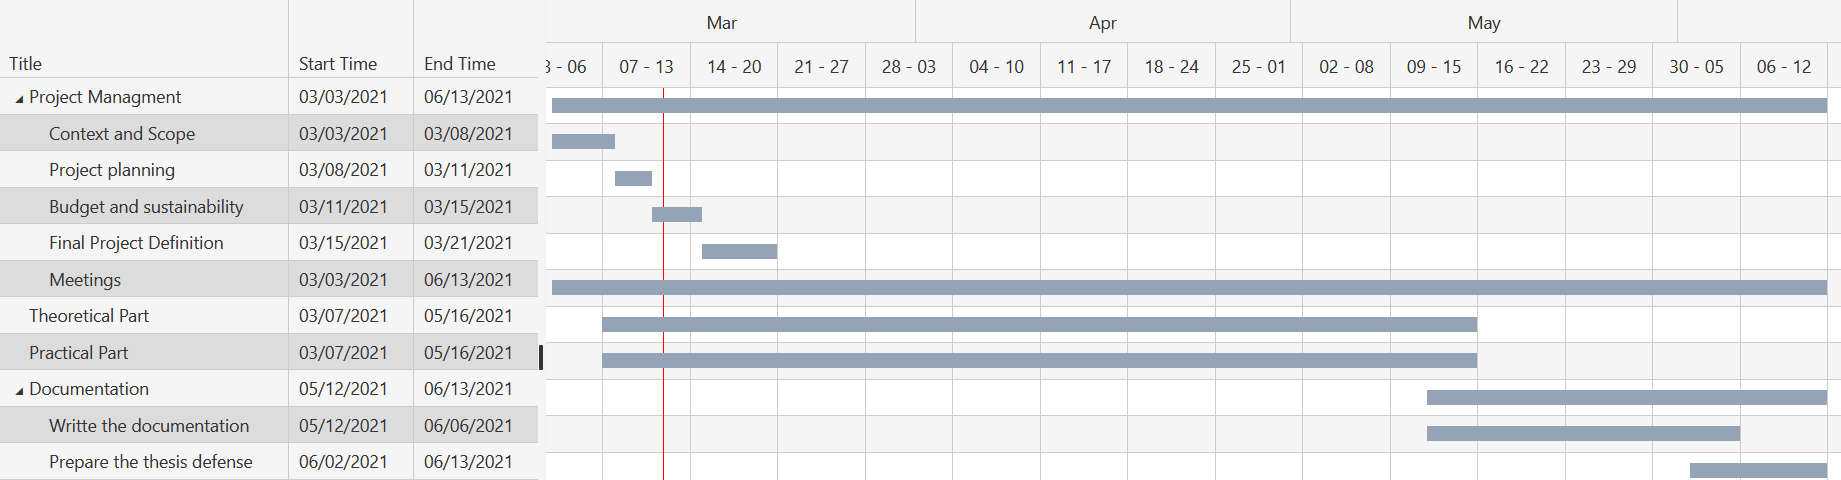
\includegraphics[scale=0.35]{img/gantt.png}
    \caption{A summary of the tasks represented with a gantt chart. Notice that all the theoretical and practical tasks are done in parallel.}
    \label{fig:gantt}
\end{figure}

\section{Resources}

Our project needs resources to carry out its correct development. These resources have been divided in 4 different groups: human, hardware, software and material resources.

\subsection{Human resources}
\label{sec:human_resources}

There are three human resources that are directly involved in this project.

\begin{itemize}
    \item \textbf{The researcher:} He is responsible for the development of the project, that is, he will have to plan, analyze, program, experiment and document the project.
    \item \textbf{The director/tutor:} He is responsible for leading and guiding the researcher for the correct development of the project.
    \item \textbf{The GEP tutor:} He is in charge of reviewing the project management tasks done in the initial stage of the project.
\end{itemize}

\subsection{Hardware Resources}
\label{sec:hardware_resources}

The most essential resource needed is a computer connected to the internet. In this project a personal computer will be used. Its specializations are 16 GB of RAM and a CPU \emph{AMD Ryzen 7 4800HS}, with a base speed of 2.9 GHz and 8 cores. Hardware required for a connection to the internet (a router, an access point, etc) is also taken into account.

\subsection{Software Resources}

For project management tasks \texttt{Google Calendar} will be used. A number of other Google products such as \texttt{Google Mail}, \texttt{Google Drive} or \texttt{Google Meet} will also be used as tools required for communication with the director or storing of information.

The documentation will be written with \LaTeX, a document preparation system often used in academia. It has the advantage to integrate well with version control systems. A \LaTeX \ template named "\texttt{Masters/Doctoral Thesis}" will be used to facil\-itate the type\-setting and styling of the document. This template was made by Vel and Johannes Böttcher and licensed under \texttt{LPPL 1.3}, based on previous work from Steve R. Gun and Sunil Patel and used with minor modifications. The original is available at \url{http://www.latextemplates.com/}. The document will be written with the \texttt{Microsoft Visual Studio Code} editor, using the \texttt{LaTeX Workshop} extension, and it will be compiled with the \texttt{MiKTex} distribution installed on a \texttt{Linux} machine run\-ning virtualized within a \texttt{WSL} container on top of the actual operating system, a \texttt{Microsoft Windows 10}. For browsing the internet the latest available version of the \texttt{Mozilla Firefox} web browser will be used, and references to papers will be kept with the \texttt{Zotero} reference manager.

For the practical part the programming language of choice will be \texttt{Python3}. This is currently one of the programming languages with better popularity in machine learning and related applications. Various libraries and software packages will be used for different tasks. For parsing datasets the \texttt{pandas} library will be used. For data visualization the \texttt{mathplotlib} library will be used. Also, a general tool-set designed for machine learning, the library \texttt{sklearn}, will be used. Finally, code will be documented in-place during its development with the \texttt{Jupyter Notebook} software.

Other libraries and software packages could also be used if the need arises. 

\subsection{Material Resources}

In a research focused project such as this, access to scientific journals, books and similar research material is needed. Some articles related to this research are freely available on the internet but some require a subscription or single time payment. Fortunately, the UPC, the University this project is being developed at, has a sub\-script\-ion agree\-ment with most of these journals and provides free access to their members, including the students.


\section{Risk Management}
\label{sec:risk_management}
The potential risks and obstacles have already been introduced in section \ref{sec:risk}. In this section we will focus on a contingency plan to mitigate the risks.

\begin{itemize}
    \item \textbf{Deadline of the project:} The flexibility of the Kanban methodology should help us modify our schedule and working hours if required. If it becomes apparent that the deadline will not be meet, that is, more than 50 hours a week of work are required to finish the project in time, an extension of the deadline can be requested.
    \item \textbf{Bugs on some libraries:} Alternative libraries can be used. If no alternative is found, because most of the used libraries are open source, a \emph{bugfix} could be implemented. 
    \item \textbf{Insufficient computational power:} This can be mitigated by using a small sample of the data-set. Working with fewer data, although faster, can induce a small performance reduction and make the results not comparable with each other. Therefore, this solution is not ideal. 
    \item \textbf{Hardware related issues:} To avoid data loss, all code and documentation will be routinely uploaded to the cloud in a \texttt{GitHub} repository and \texttt{Google Drive} account.
    \item \textbf{Health related issues:} Not much can be done if a health related problem occurs, but various preventive actions, such as a good diet, exercise and resting habits can be promoted.
\end{itemize}





% Chapter 3

\chapter{Budget and Sustainability} % Main chapter title
\label{Chapter3}

In this section a budget estimation will be made. It will include personnel costs per task, generic costs and other costs. Moreover, some questions regarding the sustainability aspect of the project will be answered.

\section{Budget}
\label{sec:budget}

\subsection{Costs by role and activity}

In this section we will add the personnel costs to the tasks defined in section \ref{sec:tasks}. For each task a cost will be calculated based on the hourly pay wage per role and the time spend each. Four roles have been defined with their corresponding hourly wage, these are:

\begin{itemize}
    \item The \textbf{project manager} (T1) who is responsible for leading the project direction, planning and correct development.
    \item The \textbf{researcher} (T2), who must perform research in the topic and related ideas, experiment, analyze the results and draw conclusions from them.
    \item The \textbf{programmer} (T3), who must set up the developer environment, code the algorithms in the specified programming language and test them for cor\-rect\-ness.
    \item The \textbf{technical writer} (T4), who is responsible for writing this project doc\-u\-men\-ta\-tion. This includes the reports for each task that requires it and the final thesis.
\end{itemize}

These roles have a clear mapping to the task groups defined in table \ref{tab:tasks}. All roles will be played by the researcher (see section \ref{sec:human_resources}) except the project manager role, which will be played by the researcher, the director and the GEP tutor. For a detailed description of each task cost see table \ref{tab:task_cost}.

Notice that, although we aligned the project roles with the task groups so that we could simplify our calculations, it is not required to do so. A more complicated scheme where multiple tasks are assigned to a given role is also possible. In such cases we would also have to think about weather the work distribution is uniform or not, and assign percentages if it isn't.

\newpage

\begin{table}[h]
    \centering
    \begin{tabular}{l c c c c r}
    \toprule
    \tabhead{Role} & \tabhead{Year (\euro)} & \tabhead{Year +SS (\euro)} & \tabhead{Hour +SS (\euro)} & \tabhead{Task} & \tabhead{Task Cost (\euro)} \\
    \midrule
    Project Manager & 39 000 & 50 700 & 28.7 & T1 & 2 296 \\
    Researcher & 32 000 & 41 600 & 23.5  & T2 & 3 760\\
    Programmer & 26 000 & 33 800 & 19.1  & T3 & 3 065\\
    Technical writer & 22 000 & 28 600 & 16.2 & T4 & 1 260 \\
    \midrule
    \textbf{Total} & & & & & \textbf{10 381} \\
    \bottomrule\\
    \end{tabular}
    \caption{Annual estimated salary for the different project roles  (\cite{noauthor_salarios_2017}). The amount of working hours in a year is defined to be 1764. \emph{+SS indicates “Social Security included”}.}
    \label{tab:task_cost}
\end{table}

\subsection{Generic costs}

\subsubsection*{Amortization}

In this section the amortization costs for the resources purchased in a single payment are calculated. Notice that since all the software used is free and open source, it doesn't contribute to the cost, thus it is not displayed here. In fact, the only resource that is valid for an amortization analysis is the computer specified in section \ref{sec:hardware_resources}.

The equation we use to compute the amortization cost for each resource is the following:

\begin{equation}
    \text{Amortization (\euro)} = \text{Cost (\euro)} \times \frac{1}{4\text{ years}} \times \frac{1}{100\text{ days}} \times \frac{1}{5\text{ hours}} \times \text{Hours Used}  
\end{equation}

If we apply the amortization equation to the computer, which we purchased for \euro999.95, and assuming 500 hours of usage, its estimated amortized cost is \euro249.98.

\subsubsection*{Electric cost}

In this section we only calculate a rough estimate. Calculating accurately the cost of electricity involves many variables, and it's outside the scope of this thesis. The average cost of electricity in Spain, in therms of kWh, is \euro0.12. We only count the cost when the hardware is turned on. The following table (\ref{tab:electric_cost}) shows the individual and total cost per item.

\begin{table}[h]
    \centering
    \begin{tabular}{l c c c r}
    \toprule
    \tabhead{Item} & \tabhead{Power (W)} & \tabhead{Time used (h)} & \tabhead{Consumption (kWh)} & \tabhead{Cost (\euro)} \\
    \midrule
    Computer & 180 & 500 & 90 & 10.8 \\
    Router & 10 & 500 & 5 & 0.6 \\
    \midrule
    \textbf{Total} & & & & \textbf{11.4} \\
    \bottomrule
    \end{tabular}
    \caption{Electric cost estimate.}
    \label{tab:electric_cost}
\end{table}

\subsubsection*{Internet cost}

The internet cost in my current location is \euro29.00 per month, this is roughly about \euro0.95 per day (variance is introduced because a month length is not constant). The amount of working hours per day is assumed to be 5, thus the total cost the whole project is:

$$
\text{\euro}0.95\text{ /day} \times 100 \text{ days} \times 5/24 \text{ hours} = \text{\euro}19.79
$$

\subsubsection*{Work space}

This project will be developed at my parents home at Figueres, with a rent of \euro400. Since the amount of people living there is 2, the actual cost is \euro200.

\subsubsection*{Total generic costs}

Table \ref{tab:generic_cost} summarizes the total generic costs of this project.

\begin{table}[h]
    \centering
    \begin{tabular}{l r}
    \toprule
    \tabhead{Group} & \tabhead{Cost (\euro)} \\
    \midrule
    Amortization & 249.98 \\
    Electricity & 11.4 \\
    Internet & 19.79 \\
    Rent & 200 \\
    \midrule
    \textbf{Total} & \textbf{481.17} \\
    \bottomrule
    \end{tabular}
    \caption{Total generic cost estimate.}
    \label{tab:generic_cost}
\end{table}

\subsection{Other costs}

\subsubsection*{Contingencies}

Unexpected problems that were not foreseen may appear during the development of the project, which would take part of our budget. For this reason it as always a good idea to prepare a contingency budget calculated from the budgets we've calculated up to now. We will apply a 10\% contingency margin, that is \euro108.62.

\subsubsection*{Incidental cost}

Unexpected problems that were foreseen and can be mitigated are described in section \ref{sec:risk_management}. Some of these mitigations may incur some extra cost. To be able to handle that cost in this section we will calculate a budget based on the predicable problems, their chances of actually occurring, and the expected cost associated for solving them.

\begin{itemize}
    \item \textbf{Deadline of the project:} If an extension of the deadline is requested, that would require extra hours expend by the researcher. Assuming the extra time required to be 50 hours that would give us a cost of \euro1,175.
    \item \textbf{Bugs on some libraries:} Implementing a \emph{bugfix} we assume would cost around 20 hours, a task done by the programmer. The estimated cost is \euro382. The risk is small.
    \item \textbf{Insufficient computational power:} If using smaller datasets where not an option, we would abandon the project, since purchasing a new, more powerful, computer or renting a supercomputer is too expensive. The risk is very small.
    \item \textbf{Hardware related issues:} New hardware would be purchased, if possible only the faulty component would be replaced. This would have an estimated cost of about \euro100. The risk is small.
\end{itemize}

The following table summarized the expected cost due to foreseen incidents.

\begin{table}[h]
    \centering
    \begin{tabular}{l r r r}
    \toprule
    \tabhead{Risk} & \tabhead{Expected (\euro)} & \tabhead{Risk (\%)} & \tabhead{Cost (\euro)} \\
    \midrule
    Deadline of the project & 1 175 & 30 & 352.5 \\
    Bugs on some libraries & 382 & 10 & 38.2 \\
    Insufficient computational power & & 5 &  \\
    Hardware related issues & 100 & 10 & 10 \\
    \midrule
    \textbf{Total} & & & \textbf{400.7} \\
    \bottomrule
    \end{tabular}
    \caption{Total incidental cost estimate.}
    \label{tab:incident_cost}
\end{table}

\subsection{Total cost}

The total cost for the project is summarized in table \ref{tab:total_cost}. The cost has been computed as the sum of the justified costs explained in the other sections of the budget plan.

\begin{table}[h]
    \centering
    \begin{tabular}{l r}
    \toprule
    \tabhead{Section} & \tabhead{Cost (\euro)} \\
    \midrule
    Costs by role and activity & 10 381.00 \\
    Generic costs & 481.17 \\
    Other costs & 509.32 \\
    \midrule
    \textbf{Total} & \textbf{11 371.49} \\
    \bottomrule
    \end{tabular}
    \caption{Total cost estimate.}
    \label{tab:total_cost}
\end{table}

\section{Sustainability}

This project does not have a major environmental impact, since it's a re\-search project. Still, some impact, a very small amount, is expected from the electricity consumption and hardware used. This can hardly be reduced, as is required for the development of the project. If the project succeeds at finding improvements to the SVM-RFE al\-go\-rithm, it will reduce computing power requirements for future researches that use it compared to the state-of-the-art solutions. Because this algorithm is used in medical research, a substantial improvement could create a chain reaction that benefits the health of the population in general. This, however, is a very optimistic expectation.

\subsection{Environmental dimension}

\subsubsection*{Have you estimated the environmental impact of undertaking the project?}

This project will not have a major environmental impact. Still, some impact, a very small amount, is present in the form of electricity consumption and the method used by the provider to generate such electricity. Also, the hardware used will eventually contribute to the technological waste problem, not to mention the environmental cost for their production.

\subsubsection*{Have you considered how to minimize the impact, for example by reusing re\-sources?}

The impact is directly derived from the project requirements and can thus not be reduced easily. A low-cost computer doesn't necessarily imply a lower impact on the environment or lower electricity consumption. Recycling is of course always an option, but the decision to do so will be taken way after the project has been completed.

\subsubsection*{How is the problem that you wish to address resolved currently (state of the art)? In what ways will your solution environmentally improve exist\-ing solutions?}

This project will use the same resources as those used in state-of-the-art alternatives. Therefore, this solution does not environmentally improve existing solutions. If the project succeeds at finding an improvement to the SVM-RFE algorithm however, it could imply a reduction on computational power required to solve some problems, and thus also a reduction in power consumption.

\subsection{Economic dimension}

\subsubsection*{Have you estimated the cost of undertaking the project (human and material re\-sources)?}

Yes, see section \ref{sec:budget}.

\subsubsection*{How is the problem that you wish to address resolved currently (state of the art)? In what ways will your solution economically improve existing solutions?}

If improvements to the SVM-RFE are found in this project, this will make any re\-search that makes use of it less expensive and produce better results.

\subsection{Social dimension}

\subsubsection*{What do you think undertaking the project has contributed to you personally?}

This is the last step required to finish my degree in computer science. Finalizing this degree will allow me to enter the work force and become self-sufficient. Beyond that, it has introduced me to the fields of bioinformatics and data mining, as well as shown the importance of feature analysis and how it can be not just a cleaning prerequisite for a more important problem, but the main dish. 

\subsubsection*{How is the problem that you wish to address resolved currently (state of the art)? In what ways will your solution socially improve (quality of life) existing. Is there a real need for the project?}

Improvements to the SVM-RFE algorithm may or may not be found. Even if found it is still unknown if they will be substantial enough. Moreover, an analysis of the variants of the algorithm will be useful for those who want to use SVM-RFE in the most optimal way.

\chapter{Background}
\label{Chapter4}

In this section we're going to review the concepts required to understand the SVM-RFE algorithm. Section \ref{sec:context} already introduced some concepts around the SVM-RFE algorithm, placed it in context, and enumerated some of its applications. In this section we'll focus on the inner workings of the algorithm and how these parts add together. 

\section{Machine learning}

Machine learning is a subfield in the broader discipline that is artificial intelligence, with a particular take in statistics. These algorithms, also called learning machines or just machines, use data to learn patterns and make predictions. The data is collected in a separated unrelated process, and structured in the form of a \emph{dataset} (a collection of data). Once the dataset is further cleaned and prepared, the learning machine finally consumes it in a process called \emph{training}. After this process the machine pro\-duces a \emph{model}, which is a function that can be used to make predictions on new data.

Two canonical problems in machine learning are regression and classification problems.

\subsection{The dataset}

A dataset is simply a collection of data. In the context of machine learning this data-set will be used to make predictions, take decisions, or find patterns. For a machine learning algorithm to be able to consume a dataset the first step is to represent it in tabular form. 

Most datasets come already in tabular form. Some of the most notable ex\-cep\-tions are datasets involving images. In this case computer vision methods are often used to extract numeric data representing characteristics of the image. Sometimes a more direct transformation can also be made, for example making each feature be the intensity level of a single pixel in the image. This of course produces a high number of features, most of which are redundant or irrelevant (e.g. features representing pixels in the background). 

In a dataset represented as a table, columns describe different \emph{features}, \emph{properties} or \emph{attributes} of some group of objects and rows represent \emph{instances} or \emph{examples} of that group. For example, if objects were vehicles then features could include the brand, power, weight, max\-imum speed, and other such characteristics of various vehicles, each of which would be in a row. Different names are used in different contexts. One of the most typical naming conventions comes from the statistics domain which refers to columns as \emph{variables} and rows as \emph{observations}. Sometimes different nomenclature is used to differentiate features in different stages of the cleaning and preparation process, but in this thesis we use them all instinctively.

\begin{table}[h]
    \makebox[\textwidth][c]{
        \begin{tabular}{l l l l l l l l l}
        \toprule
        \tabhead{Src} & \tabhead{Dst} & \tabhead{NAT-Src} & \tabhead{NAT-Dst} & \tabhead{Action} & \tabhead{Sent (B)} & \tabhead{Rcvd. (B)} & \tabhead{Packets} & \tabhead{Elapsed (sec)}\\
        \midrule
        57222 & 53 & 54587 & 53 & allow & 94 & 83 & 2 & 30 \\
        56258 & 3389 & 56258 & 3389 & allow & 1600 & 3168 & 19 & 17 \\
        6881 & 50321 & 43265 & 50321 & allow & 118 & 120 & 2 & 1199 \\
        43537 & 2323 & 0 & 0 & deny & 60 & 0 & 1 & 0 \\
        50002 & 443 & 45848 & 443 & allow & 6778 & 18580 & 31 & 16 \\
        \bottomrule\\
        \end{tabular}
    }
    \caption{Example dataset extracted from the Internet Firewall Data (\cite{ertam_internet_2019}). Only five observations and main variables shown. }
    \label{tab:example_dataset}
\end{table}

\subsection{Classification}
\label{sec:ch4.classification}

For the classification problem we want to predict in witch group or \emph{class} to assign some new observation. Table \ref{tab:example_dataset} provides an example of what could be a good classification problem. Imagine we are building a firewall and want it to predict if some new packet in the network should be allowed to pass. We could train a classification learning machine with the dataset represented in the table (the full version) and produce a model capable of doing such predictions. Although it is trivial to identify a pattern in the example, it may not be so for real world examples. Automatic \emph{pattern recognition} is key in solving many real world problems, and it is one of the features of these algorithms.

Mathematically, the set of observations is defined as $X = \{\vt{x_1}, \vt{x_2}, \dots, \vt{x_n}\}$ and the set of the corresponding labels or target classes is $y = \{y_1, y_2, \dots, y_n\}$ with every element of this set being some class $y_i = C_k$ of a discrete set of classes with size $K$. They are called \emph{domain set} and \emph{label set} respectively. For our example, the classes would be $C = \{\text{allow}, \text{deny}\}$. Thus, we can describe the goal of a classification problem as assigning some class $C_k$ to an input vector $\vt{x}$.

Although we've used strings to represent classes, part of the preparation process of the dataset involves turning all values into numerical scalars, so our classes would actually be some natural numbers. Also notice that every $\vt{x_i}$ is a vector containing a single numerical value for each feature excluding the label. 

We make a distinction between two-class problems (or binary) and multi-class problems. Two-class problems typically use $C = \{0, 1\}$ as classes and thus can be modeled with a boolean function or, if a probability is desired, a function that returns values between 0 and 1. This simplifies the model substantially, in fact some learning machines such as the SVM can only work with two-class problems, and use different methods to extend to the multi-class version.

\subsection{Visualization}
\label{sec:ch4.visualization}

A visualization of the problem in some euclidean space is required to understand how most classification algorithms work, and in particular SVM. Typically, clas\-si\-fi\-cation models divide the input vector space\footnote{The euclidean space of minimum dimension containing all possible input vectors $\vt{x}$.} into \emph{decision regions}. The boundaries of such regions are called \emph{decision boundaries} or \emph{decision surfaces}. If the decision boundary is in the form of some hyperplane of dimension $(D - 1)$, with $D$ being the dimension of the space, then we say that it's a linear model. A dataset whose classes can be completely separated by such linear decision boundary is said to be \emph{linearly separable}.

\begin{figure}[H]
    \centering
    \begin{subfigure}[b]{0.4\linewidth}
        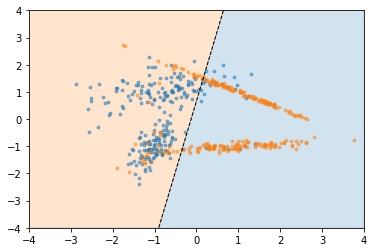
\includegraphics[width=\linewidth]{img/ch4/nolinsep.png}
        \subcaption*{Not linearly separable}
    \end{subfigure}
    \begin{subfigure}[b]{0.4\linewidth}
        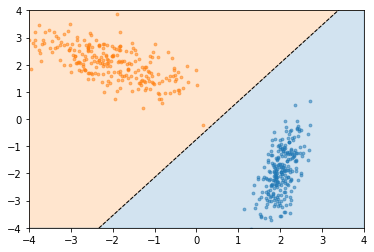
\includegraphics[width=\linewidth]{img/ch4/linsep.png}
        \subcaption*{Linearly separable}
    \end{subfigure}
    \caption{Decision regions and 1-D hyperplane boundary of some linear model for two datasets. Points are observations, colors indicate the class.}
    \label{fig:ch4.sep}
\end{figure}

Given a boundary we can determine in which region some new point $\vt{x}$ falls using a \emph{discriminant function}. One of the most trivial cases is when the boundary is lineal. It is convenient now to do a small refresh on the equation that describes a hyperplane.

\subsubsection*{Equation of a line (slope-intercept form)}
\begin{align}
    y = mx + t
\end{align}

Where $m$ is the \emph{slope} or \emph{gradient}, $x$ is the independent variable of the function $y = f(x)$ and $t$ is the y-intercept value, the point of the function where the line crosses the y-axis, i.e. $t = f(0)$. This description has the advantage that can be directly represented as a function $f(x) = mx + t$.

\subsubsection*{Equation of a line (standard form)}
\begin{align}
    ax + by = c
\end{align}

This is an equivalent form, this one however is not representable by a function $f: \mathbb{R} \rightarrow \mathbb{R}$, instead it is often represented as a set $L = \{(x, y) \st ax + by = c\}$. This allows representing vertical lines and also features the useful property that $(a, b)$ is the normal vector\footnote{A vector that is perpendicular to the surface.} of the line.

\subsubsection*{Equation of a line (general form)}
\begin{align}
    ax + by - c = 0
\end{align}

A simple linear transformation of the standard form produces the general form (\cite{noauthor_wikipedia_2021}). This conserves the normal vector and also has the advantage of being representable by an implicit function\footnote{A function of multiple variables $f: \mathbb{R}^n \rightarrow \mathbb{R}$ such that we only consider solutions where $f(X) = 0$. For example a circle can be defined with an implicit function $f(x, y) = x^2 + y^2 - r$, but if we were to plot it in 3-D we would instead see an inverted cone.}. Notice that if represented in 3-D it would produce a plane that is perpendicular to the $xy$ plane, since its normal would always have the form $(a, b, 0)$.

\subsubsection*{Equation of a 3-D Plane}
\begin{align}
    ax + by + cz + d = 0
\end{align}

We can extend the general form of a line with one more dimension, it only requires adding the new term $cz$ for the new dimension. We've also changed the sign of the constant term $d$ for compactness. This is a conceptual move, not an algebraic one.

\subsubsection*{Equation of a Hyperplane}
\begin{align}
    w_1x_1 + \dots + w_nx_n + w_0 = 0
\end{align}

This is a generalization of the equation of a 3-D plane for $n$ dimensions. It also happens to be the definition of a \emph{linear equation}. The variables $w_1, \dots, w_n$ are called \emph{coefficients}, \emph{parameters} or \emph{weights}, and the variable $w_0$ is the constant term. It is important to avoid confusing $x_i$ with $\vt{x_i}$, the first is the one the coordinates of a point in some dimension, and the other is an observation of a dataset (a point). In particular, it may be the case that $\vt{x_j} = (x_1, x_2, \dots, x_n)$.

We may want to compact this expression more by using vectors. So, another form for representing the equation of a hyperplane is:
\begin{align}
    \vb{w}^{\T}\vb{x} + w_0 = 0
\end{align}

Where $\vb{w}$ is called the \emph{vector weight} and $w_0$ the \emph{bias}. We can turn this equation into a discriminant function for two classes by simply considering what happens with points that are not in the hyperplane. By definition such points meet one of the two inequations:

\begin{align*}
    \vb{w}^{\T}\vb{x} + w_0 > 0 \\
    \vb{w}^{\T}\vb{x} + w_0 < 0
\end{align*}

A point will be a solution of one of these inequations depending on whether it is in the subspace, i.e. discriminant region, facing the direction of the normal or the opposite.

A linear binary classification learning machine is thus an algorithm that given some dataset finds appropriate values for the parameters $\vb{w}$ and $w_0$ of the hyper\-plane in order to produce a discriminant function $y : \mathbb{R}^n \rightarrow \mathbb{R}$ such as:
\begin{align}
    y(\vb{x}) = \vb{w}^{\T}\vb{x} + w_0
\end{align}

\subsection{Performance}

Usually models produced by a learning machine do not always make correct pre\-dict\-ions, instead we consider them good enough if they can classify new data correctly most of the time. In order to quantize how good of a predictor some model is we can use various performance metrics.

The most typical metric for classification problems is \emph{accuracy}. This is the ratio of correct predictions versus the total number of predictions made. The inverse to the accuracy is defined as the \emph{error}. Notice that the classification accuracy will always be some percentage above 50\%. This is because a classifier performing consistently worse than that can be turned into a good classifier by simply flipping the output of the discriminant function. Thus, the worst possible classifier is that of a coin toss, i.e. a uniform random distribution, with an expected accuracy of exactly 50\%.

In some problems a distinction is made between misclassifications depending on which class is misclassified. An example of this is how misclassifying a patient with cancer with a healthy diagnosis is worse than misclassifying a healthy patient with a cancer diagnosis, the consequence of one is potentially death due to lack of treatment while the other is simply more investigation. For these problems a quadratic amount of cases appears. For the binary classification the standard nomenclature is to name the classes \emph{positive} and \emph{negative} and then prefix them with \emph{true} or \emph{false} depending on whether the prediction was correct or not. In this way a matrix called \emph{confusion matrix} is created, with the diagonal containing all the correct predictions.

\begin{figure}[H]
    \centering
    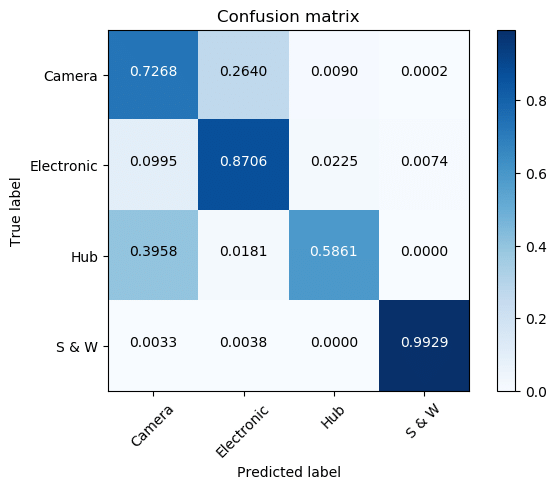
\includegraphics[width=0.5\linewidth]{img/ch4/confusion.png}
    \caption{Confusion matrix extracted from the paper “Automatic Device Classification from Network Traffic Streams of Internet of Things” (\cite{bai_automatic_2018}).}
    \label{fig:ch4.confusion}
\end{figure}

From a confusion matrix various other metrics can be extracted, such as \emph{precision}, \emph{specificity} or \emph{recall}, but it is unlikely that we make use of them in this project. Often models internally use a \emph{loss} or \emph{cost} function that they try to minimize in order to optimize the parameters, the inverse of which is called \emph{utility function}. Even if the model doesn't internally use one such function, one can be constructed form performance metrics, which is then referred as the \emph{score}. 

It is known that learning requires both \emph{generalization} and \emph{memorization}. If a model memorizes the dataset, thus has high accuracy on data already in the dataset, but doesn't generalize well, thus has low accuracy when predictions are done on new data, we say there is \emph{overfitting}. Notice that for this to be detected we must test the dataset with new data. In order to do so a dataset is often split in \emph{train} and \emph{test} subsets, and although accuracies form both subsets may be reported, only the accuracy of the test subset may be taken as good.

One of the possible causes of overfitting is the \emph{Bias-Variance} trade-off. It's an effect in which if you select a very simple model then the algorithm fails to generalize (bias) but selecting a very complex algorithm increases memorization and leads to high variability in the presence of an unseen observation (variance). The best model is thus one with a middle-ground complexity.

Selecting the complexity of an algorithm can be done with the use of some extra parameters, not fitted by the training phase of the leaning machine, that we call \emph{hyper-parameters}. The existence of this extra parameters depends on the models, some may not have any. Because these parameters modify the model, searching for the best hyper-parameters is called \emph{model selection}. Model selection is often done in a brute force manner, by simply trying different values of the hyper-parameters and selecting the ones that give the best result. Al\-though this coarse strategy is usually enough, more complex search strategies such as successive halving or genetic algo\-rithms (\cite{claesen_hyperparameter_2015}) can also be used. In the case of one single hyper-parameter we can draw a plot and visualize how the score evolves. Because model selection may be understood as some kind high level training, specially when com\-plex search strategies are used, a third division on the dataset may be made, named the \emph{validation} set.

\begin{figure}[H]
    \centering
    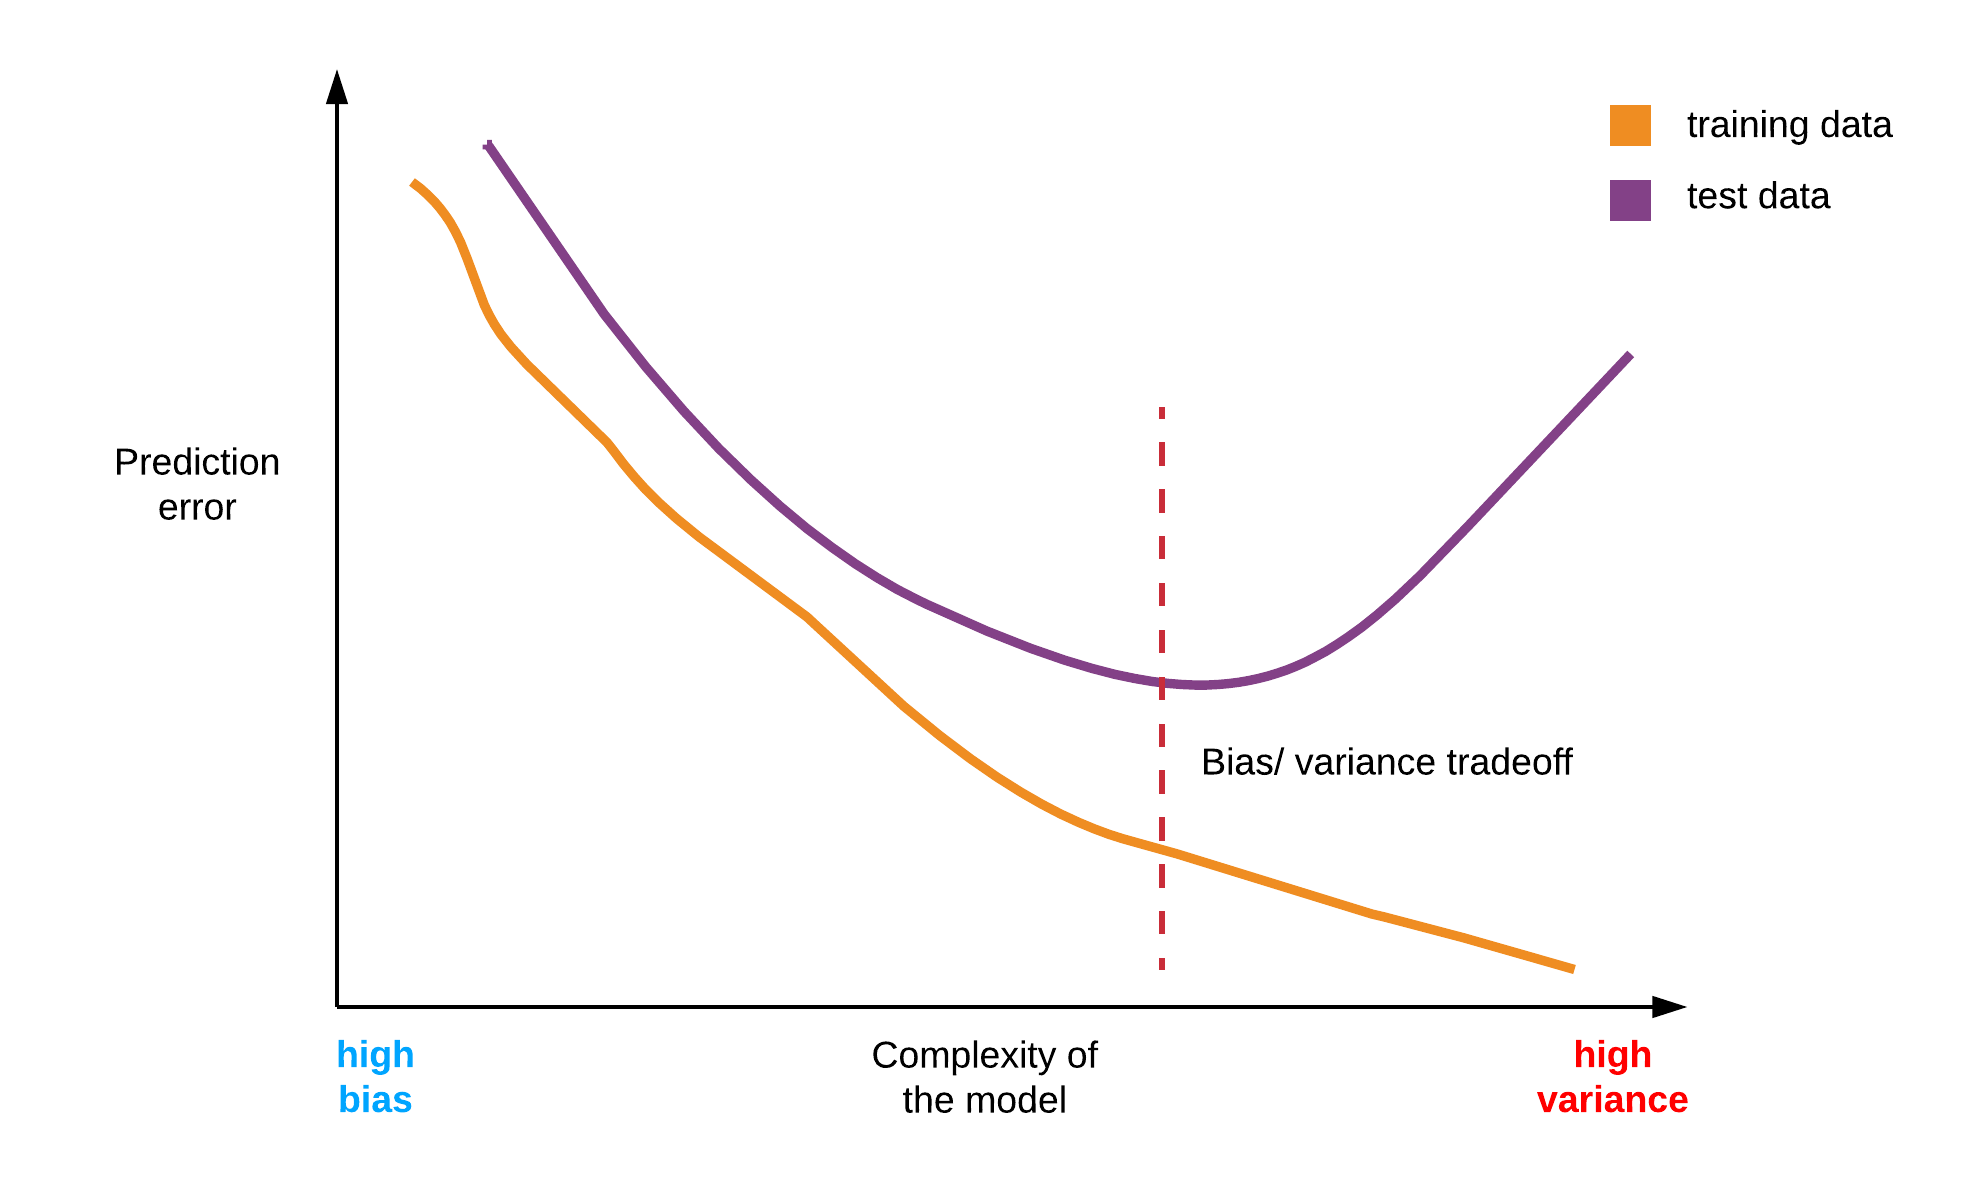
\includegraphics[width=0.5\linewidth]{img/ch4/bias-and-variance.png}
    \caption{Bias-Variance trade-off. Source (\cite{bisong_machine_2021}).}
    \label{fig:ch4.biasvariance}
\end{figure}

Machine learning algorithms work better the more observations they are trained with, however it is not often the case that we have an unlimited amount of them. In analyzing the performance of a leaning machine, or doing model selection, it may be useful to repeat the experiments multiple times with different data of the same distribution, i.e. from the same dataset. This provides second order statistics, such as the mean or the covariance, on the resulting scores, which may prove very useful to get a better idea of what is going on. This however implies further slicing the dataset in as many slices as experiments one wants to do. After so much slicing, the remaining training subsets would often contain very few observations, thus reducing the performance of the models and nullifying the advantages of having a probability distribution on the scores. 

A method called \emph{cross-validation} can be used to make mul\-ti\-ple experiments with\-out increasing the amount of data. The method first makes $K$ partitions called \emph{folds}. For each fold, one experiment is made such that the fold is used as the validation set and the remaining folds become the training set. This allows a portion $(K-1)/K$ of the observations to be used for training in each run and allows assessing performance using the whole dataset. In the particular case where $K = N$, useful for when the amount of observations is really low, we name this method \emph{leave-one-out} cross-validation. It is also possible to shuffle the data, which allows even more re-utilization. Although this method is computationally expensive (since it requires running the whole experiment $K$ times), it has the advantage of being trivial to parallelize, and thus it can run at increased speeds in computers with a multi-core CPU architecture. 

\section{Support Vector Machines}

As it has been discussed in section \ref{sec:ch4.visualization}, the decision boundary of a binary class\-ification prob\-lem may be represented with a hyperplane, and it is the weights of this hyperplane what the learning machine tries to fit such that the hyper\-plane correctly separates the two classes. There may be infinitely many hyperplanes that correctly separate the examples of two classes, but some of them are better suited than others. For the purpose of generalization, we want decision regions that can accommodate new data outside the convex hulls\footnote{In geometry, the \emph{convex hull} or \emph{convex envelope} of a shape is the smallest convex set that contains it.} of each group of examples. That is, we want some kind of separation between the hyperplane and the observations.

\begin{figure}[H]
    \centering
    \begin{subfigure}[b]{0.4\linewidth}
        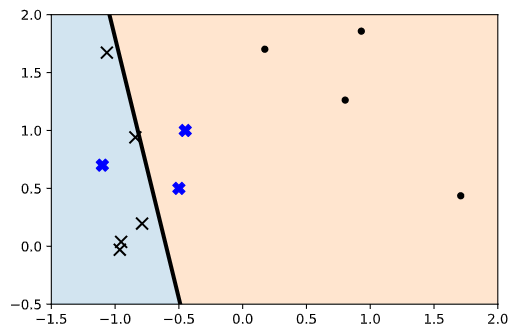
\includegraphics[width=\linewidth]{img/ch4/boundrybad.png}
        \subcaption*{Bad boundary}
    \end{subfigure}
    \begin{subfigure}[b]{0.4\linewidth}
        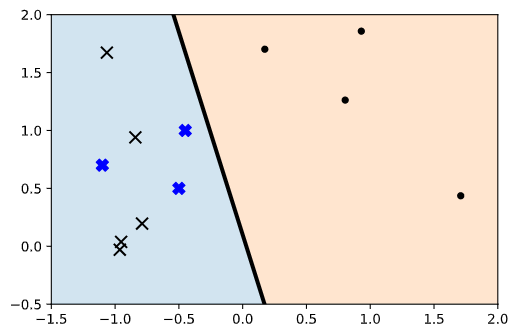
\includegraphics[width=\linewidth]{img/ch4/boundrygood.png}
        \subcaption*{Good boundary}
    \end{subfigure}
    \caption{Showing how one decision boundary may be better than another. \texttt{X} filled in blue represents new data.}
    \label{fig:ch4.sep}
\end{figure}

There exist various learning machines that accomplish this separation, e.g. the \emph{Fisher’s linear discriminant}. Another such machine is the Support Vector Machine (SVM), which is based on the idea of finding the biggest margin between the extreme points of each class and setting the decision boundary in the center of such margin. For this reason SVM machines are said to be \emph{Maximum Margin Classifiers}.

\begin{figure}[H]
    \centering
    \begin{subfigure}[b]{0.4\linewidth}
        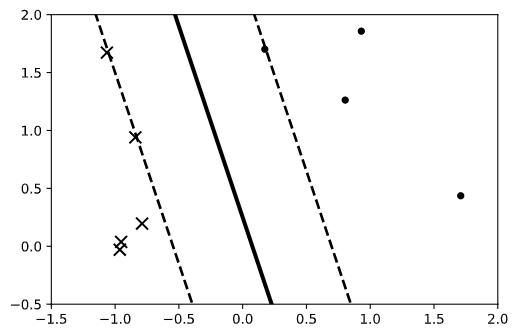
\includegraphics[width=\linewidth]{img/ch4/mmc_good.png}
        \subcaption*{Maximum margin}
    \end{subfigure}
    \begin{subfigure}[b]{0.4\linewidth}
        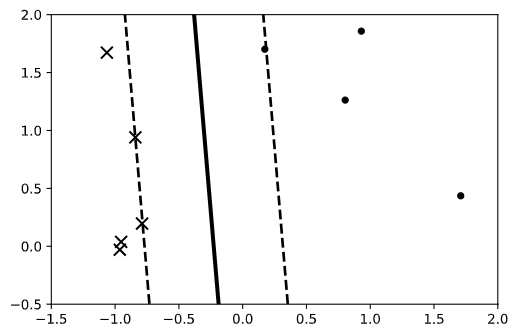
\includegraphics[width=\linewidth]{img/ch4/mmc_bad.png}
        \subcaption*{Quite good margin}
    \end{subfigure}
    \caption{Two quite good decision boundaries with a margin, a maximum margin classifier would choose the left one.}
    \label{fig:ch4.sep}
\end{figure}

The \emph{margin} is defined as the perpendicular distance (i.e. in the direction of the normal) between the decision bound\-ary and the closest of the examples. There is only one decision boundary that maximizes the margin. Only a limited amount of examples, defined by the number of dimensions, will reach the limits of that margin (and thus be the closest), these are called the \emph{support vectors}.

\subsection{Discriminant function}

We've already seen how to we can build a discriminant function from the equation of the hyperplane. Here we will explore this in a bit more depth and take a different approx. 

Given a vector of unknown length $\vt{w}$ that is perpendicular to the hyperplane (thus the normal) such that its origin is at the origin of the coordinate system. And given another vector $\vt{x}$ also with origin at the origin of the coordinate system. Notice that, by how we are defining them, they are actually points, but we may want to think of them as vectors for now. We are interested in knowing in which decision region the point $\vt{x}$ is placed.

To do so, we make the dot product between $\vt{w}$ and $\vt{x}$, which, in particular, will give us a scalar corresponding to the length of the projection of $\vt{x}$ over $\vt{w}$. Notice that for points within the hyperplane that length will be some constant value $c$. Thus, we can know if point $\vt{x}$ is in one region or another by comparing it with $c$. This can be expressed with the inequality $\vt{w} \cdot \vt{x} \ge c$. By making a variable $b = -c$ and expressing the dot product as a product of matrices, we can conveniently rearrange this equation as the decision rule:
\begin{align}\label{eq:drule}
    \vb{w}^\T \vb{x} + b \ge 0
\end{align}
This is analogous to the decision rule found in section \ref{sec:ch4.visualization}, in fact if we make an equality instead of an inequality we discover the equation of the hyperplane, from there we could do the process in reverse until we find the general equation of a line. 

\subsection{Margin formalization}

Notice from equation \ref{eq:drule} that the constant value of $b$ depends directly on the length $||\vt{w}||$, and because this length is not limited (there are infinite vectors that are normal to the hyperplane), an infinite amount of combinations exists.

Therefore, we may want to restrict the decision rule to a single combination. Also, it is convenient that this restriction takes such a form that allows defining the margin. First we assign to our classes the numerical values $C = \{-1, 1\}$. Then we impose the condition that points in a decision region outside the margin must have values greater than $\pm 1$, thus for points $\vb{x}_{(+)}$ in class “$1$” and $\vb{x}_{(-)}$ in class “$-1$” we get:
\begin{align*}
    \vb{w}^\T \vb{x}_{(+)} + b &\ge 1\\
    \vb{w}^\T \vb{x}_{(-)} + b &\le -1
\end{align*}

This pair of equations can be simplified to a single equation by considering the vector $\vt{y}$ that we defined in section \ref{sec:ch4.classification}. Because of the numerical values we've assigned to the classes, it will contain elements such that every $y_i \in \{-1, 1\}$. Notice that if we multiply both sides by $y_i$ (and given that we know what the value of $y_i$ will be in each case), we can produce the single equation:
\begin{align}\label{eq:svmconstrain}
    y_i (\vb{w}^\T \vb{x_i} + b) \ge 1
\end{align}

From this equation we may find the values of the hyperplanes that border the margin (named \emph{gutter}), that is, the points where the last equation is exactly 1. 

\subsubsection*{Equation of the gutters}
\begin{align}\label{eq:gutters}
    y_i (\vb{w}^\T \vb{x_i} + b) -1 = 0
\end{align}

Although now we know the equation for the gutters (analogy for the margin being a street), what we're really interested about is in the distance between them. We can calculate that distance as the diff\-erence vector form any two points in the gutters projected using the unit vector of $\vt{w}$:
\begin{align*}
    (\vt{x}_{(+)} - \vt{x}_{(-)}) \cdot \frac{\vt{w}}{||\vt{w}||}
\end{align*}

Notice that form equation \ref{eq:gutters} we can derive $\vt{w} \cdot \vt{x}_{(+)} = 1 - b$ and $\vt{w} \cdot \vt{x}_{(-)} = b - 1$, applying the distributive property we obtain:
\begin{align*}
    \frac{(1 - b) - (b - 1)}{||\vt{w}||} \implies \frac{2}{||\vt{w}||}
\end{align*}

Since we've defined the margin to be the distance from the decision boundary to a gutter (i.e. where support vectors are), and since the decision boundary is at the same distance to both gutters, then we can see that the length of the margin will be half the distance between the gutters.

\subsubsection*{Length of the margin}

\begin{align}
    \frac{1}{||\vt{w}||} = \frac{1}{\sqrt{\vb{w}^\T \vb{w}}}
\end{align}

\subsection{Optimization problem}

The problem of finding the greatest margin can be formulated as an optimization problem. Specifically we want to maximize $1/||\vt{w}||$ subject to the constraints defined in equation \ref{eq:svmconstrain}. This is equivalent to minimizing $||\vt{w}||$ subject to the same constraints. For mathematical convenience (which we will see later), we can also divide by 2 and square the objective function without it affecting the optimal solution.

\subsubsection*{Primal form}
\begin{align}\label{eq:svm_primal} 
    \underset{\vt{w}, b}{\text{arg} \min}\ \frac{1}{2} ||\vt{w}||^2 \text{\quad s.t. \quad} \forall i : y_i (\vb{w}^\T \vb{x_i} + b) - 1 \ge 0
\end{align}

This is a constrained quadratic optimization problem. There are various known algorithms that can solve constrained optimization problems, such as the \emph{simplex} algorithm. However, in our case it may be appropriate to use the \emph{Lagrangian} method. This method doesn't directly return a solution, instead it transforms the problem into another version, from which a direct solution may be more easily computed.

\subsubsection*{Lagrangian}

Imagine we had an easier optimization problem. E.g. a maximization pro\-blem such that its optimization function $f : \R^{D-1} \rightarrow \R$ is a function $f(\vt{x})$ of $D$ dimensions, and it has a single equality constrain $g(\vt{x}) = 0$ of $D - 1$ dimensions. Notice how the constraint is “projected” on top of $f(\vt{x})$. Then the Lagrangian method consists on optimizing a new function (equation \ref{eq:lagrangian_base}), via introducing a new pa\-ram\-e\-ter $\lambda$ called the \emph{Lagrangian multiplier}. 
\begin{align}\label{eq:lagrangian_base} 
    L(\vt{x}, \lambda) = f(x) - \lambda g(x)
\end{align}

Notice how there is only a subset of the images of $f(\vt{x})$ for which $f$ and $g$ inter\-sect. Where the intersection is defined as $\{\vt{x} \in \R^{D-1}\ |\ \exists \vt{c} : f(\vt{x}) = c \land g(\vt{x}) = 0\}$. Many values of $c$ contribute to the intersection, however we are only interested in the maximum or minimum values, since for these $\vt{x}$ becomes a \emph{stationary point}.

An interesting property of these functions is that in the stationary points the di\-rec\-tion of the normal of both functions must be the same. Note that if the normal of $f$ was not orthogonal to the surface of $g$, we could increase $c$ by moving a short distance along the constraint surface. Also remember that the normal is the same as the gradient of that function, i.e. $\nabla f$. Therefore, there must exist a parameter $\lambda \neq 0$ (or $\lambda > 0$ for a minimization problem) such that:
\begin{align}
    \nabla f - \lambda \nabla g = 0
\end{align}

From this we see that the constrained stationary condition is obtained by setting $\nabla_x L = 0$. Notice that the gradient is defined as the partial derivatives of each coordinate in the vector, that is:
\begin{align*}
    \nabla_x L = \left( \frac{\partial L}{\partial x_1}, \frac{\partial L}{\partial x_2}, \cdots, \frac{\partial L}{\partial x_n} \right)
\end{align*}

At first glance it may look overwhelming, but given that $L$ is the same for all $x_i$ and that we can reuse the arithmetic operators for operations between vectors, doing the gradient is very similar than doing the partial derivate over a single scalar. 

Going back to the SVM formalization, we can define the Lagrangian of the primal form (equation \ref{eq:svm_primal}) as:
\begin{align}\label{eq:svm_lagrangian_from_primal}
    L(\vt{w}, b, \vt{\alpha}) = \frac{1}{2} ||\vt{w}||^2 - \sum \alpha_i \left[ y_i (\vb{w}^\T \vb{x_i} + b) - 1\right]
\end{align}

Now we want to take the partial derivative with respect to $\vt{x}$ and equal to 0. Note that $||\vt{w}|| = \sqrt{w_1^2, w_2^2, \dots, w_n^2}$, if we elevate this expression to the power of two we can eliminate the square root, then if we divide by 2 we get a vector $\left( \frac{1}{2} w_1^2, \dots, \frac{1}{2} w_n^2 \right)$ which by deviating each coordinate we get $\vt{w}$. Therefore:
\begin{align}\label{eq:svm_representer}
    \frac{\partial L}{\partial \vt{w}} = \vt{w} - \sum \alpha_i y_i \vt{x_i} = 0 \implies \vt{w} = \sum \alpha_i y_i \vt{x_i}
\end{align}

Also, by doing the gradient with respect to $b$ and comparing with 0 we get:
\begin{align}
    \frac{\partial L}{\partial b} = - \sum \alpha_i y_i = 0 \implies \sum \alpha_i y_i = 0
\end{align}
 
If we plug these expressions back in equation \ref{eq:svm_lagrangian_from_primal} we can construct the \emph{dual form}. Note that $     ||\vt{w}||^2 = \vb{w}^\T \vb{w}$.

\begin{align*}
    L &= \frac{1}{2} \left( \sum \alpha_i y_i \vt{x_i} \right) \cdot \left( \sum \alpha_j y_j \vt{x_j} \right)
    - \sum \alpha_i \left[ y_i (\vb{w}^\T \vb{x_i} + b) - 1\right]
\\
    L &= \frac{1}{2} \left( \sum \alpha_i y_i \vt{x_i} \right) \cdot \left( \sum \alpha_j y_j \vt{x_j} \right)
    - \sum \alpha_i \left[ y_i \vb{w}^\T \vb{x_i} + y_i b - 1\right]
\\
    L &= \frac{1}{2} \left( \sum \alpha_i y_i \vt{x_i} \right) \cdot \left( \sum \alpha_j y_j \vt{x_j} \right)
    - \sum \left[ \alpha_i y_i \vb{w}^\T \vb{x_i} + \alpha_i y_i b - \alpha_i \right]
\\
    L &= \frac{1}{2} \left( \sum \alpha_i y_i \vt{x_i} \right) \cdot \left( \sum \alpha_j y_j \vt{x_j} \right)
    - \sum \alpha_i y_i \vb{w}^\T \vb{x_i} - \sum \alpha_i y_i b + \sum \alpha_i
\\
    L &= \frac{1}{2} \left( \sum \alpha_i y_i \vt{x_i} \right) \cdot \left( \sum \alpha_j y_j \vt{x_j} \right)
    - \sum \alpha_i y_i \vb{w}^\T \vb{x_i} - b \sum \alpha_i y_i + \sum \alpha_i 
\\
    L &= \frac{1}{2} \left( \sum \alpha_i y_i \vt{x_i} \right) \cdot \left( \sum \alpha_j y_j \vt{x_j} \right)
    - \sum \alpha_i y_i \vb{w}^\T \vb{x_i} + \sum \alpha_i 
\\
    L &= \frac{1}{2} \left( \sum \alpha_i y_i \vt{x_i} \right) \cdot \left( \sum \alpha_j y_j \vt{x_j} \right)
    - \vt{w} \cdot \sum \alpha_i y_i \vb{x_i} + \sum \alpha_i 
\\
    L &= \frac{1}{2} \left( \sum \alpha_i y_i \vt{x_i} \right) \cdot \left( \sum \alpha_j y_j \vt{x_j} \right)
    - \left( \sum \alpha_i y_i \vt{x_i} \right) \cdot \left( \sum \alpha_j y_j \vt{x_j} \right) + \sum \alpha_i 
\\
    L &= \sum \alpha_i - \frac{1}{2} \left( \sum \alpha_i y_i \vt{x_i} \right) \cdot \left( \sum \alpha_j y_j \vt{x_j} \right)
\end{align*}

\subsubsection*{Dual form}
\begin{align}
    \underset{\vt{\alpha}}{\text{arg} \max}\ \sum \alpha_i - \frac{1}{2} \sum \sum \alpha_i \alpha_j y_i y_j \vt{x_i} \cdot \vt{x_j}
    \text{\quad s.t. \quad} \forall \alpha_i : \alpha_i \ge 0 \land \sum \alpha_i y_i = 0
\end{align}

This variation of the optimization problem has the immediate advantage of op\-ti\-miz\-ing over $\vt{\alpha}$ instead of $\vt{w}$. In cases where the number of dimensions exceeds the number of examples, solving this formulation is more efficient. Another historical reason for which the dual form has been preferred is because it allows using kernels (\cite{chapelle_training_2007}), something we will see later in section \ref{sec:ch4.kernels}.

Both this form and the primal form will require the use of a quadratic op\-ti\-miza\-tion solver. The general complexity of such algorithms is $O(n^3)$. However, various techniques can be used that accomplish to reduce this complexity for both the primal and the dual forms.

For this dual formulation, instead of directly finding the values of $\vt{w}$ we find the values of $\vt{\alpha}$. If we want to later calculate the values of the weight vector we can use the \emph{representer theorem} (equation \ref{eq:svm_representer}). For the constant parameter $b$ we can use the margin boundary equation \ref{eq:gutters}, which with some algebra can be expressed as $b = y_i - \vb{w^\T}\vb{x_i}$.

\subsection{Regularization}

Until now, we've seen how it is desirable to maximize the margin, but we've pur\-pose\-ly ignored the common situation where examples are not linearly separable. It could simply be that classes follow a distribution that is not separable using a hyperplane, in which case we would use kernels. But it could also be the case that although classes are close to be linearly separable there is some overlapping in their distributions.  

We can solve this problem by redefining our margin as a \emph{soft margin}, such that we allow some amount of observations to be incorrectly classified, thus falling within the margin or in the wrong side of the decision boundary, but with a penalty that increases with the distance to correct side of the margin. To do so we introduce \emph{slack variables}, one for each example, such that $\xi_i = 0$ if the example $i$ is correctly classified, $0 < \xi_i < 1$ if within the margin, and $\xi_i \ge 1$ if it's in the wrong side of the margin.

Now we can reformulate our \emph{primal} with this new variables, penalizing the sum of misclassifications and also introducing a \emph{regularization parameter} $C$ that allows to specify the desired trade-off strength between correct classification and slack.

\subsubsection*{Primal form with regularization}
\begin{align}\label{eq:svm_primal_reg} 
    \underset{\vt{w}, b}{\text{arg} \min}\ \frac{1}{2} ||\vt{w}||^2 + C \sum_{i=1}^{N} \xi_i
    \text{\quad s.t. \quad} 
    \forall i : y_i (\vb{w}^\T \vb{x_i} + b) \ge 1 - \xi_i \quad \land \quad \xi_i \ge 0
\end{align}

An equivalent way to perform regularization is by using an empirical risk mini\-mization approx. Given our decision rule (equation \ref{eq:drule}), we need to find a \emph{loss function} that works well for classification problems, such as the \emph{hinge loss}, defined as:
\begin{align}
    l(t) = \max \{0, 1 - t\} \text{\quad where \quad} t = y_if(x_i) = y_i (\vb{w}^\T \vb{x_i} + b)
\end{align}

This can also be written:
\begin{align*}
    l(t) = \left\{
        \begin{array}{ll}
            0   & \mbox{if} \quad t \ge 1 \\
            1-t & \mbox{if} \quad t < 1  
        \end{array}
    \right.
\end{align*}

For a given training set we seek to minimize the total loss, while regularizing the objective with $l_2$-regularization (i.e. $||\vt{w}||^2$). This gives the unconstrained reg\-u\-lar\-iza\-tion problem equivalent to equation \ref{eq:svm_primal_reg}:
\begin{align}
    \underset{\vt{w}, b}{\text{arg} \min}\ \frac{1}{2} ||\vt{w}||^2 + C \sum_{i=1}^{N} \max \{0, 1 -  y_i (\vb{w}^\T \vb{x_i} + b)\}
\end{align}

Using the same Lagrangian process shown for the hard margin version, we can obtain the dual form of the soft margin version as follows:

\begin{align*}
    L(\vt{w}, b, \vt{\xi}, \vt{\alpha}, \vt{\gamma}) = 
    \frac{1}{2} ||\vt{w}||^2 + C \sum \xi_i
    - \sum \alpha_i \left[ y_i (\vb{w}^\T \vb{x_i} + b) - 1 + \xi_i \right]
    - \sum \gamma_i \xi_i
\end{align*}

\subsubsection*{Dual form with regularization}
\begin{align}\label{eq:svm_dual_reg} 
    \underset{\vt{\alpha}}{\text{arg} \max}\ \sum \alpha_i - \frac{1}{2} \sum \sum \alpha_i \alpha_j y_i y_j \vt{x_i} \cdot \vt{x_j}
    \text{\quad s.t. \quad} \forall \alpha_i : 0 \le \alpha_i \le C \land \sum \alpha_i y_i = 0
\end{align}

This is notably similar to the hard margin version, where only one constrain has changed. 

\pagebreak

\section{Kernel Methods}
\label{sec:ch4.kernels}

The use of kernel functions enables learning machines such as SVM to have non-linear decision boundaries, thus allowing them to make correct predictions even if the dataset is not linearly separable (but separable nonetheless).

\subsection{Feature map}

A feature map is a function $\phi : D \rightarrow H$ that transforms, or maps, vectors in some space $D$ (typically $\mathbb{R}^D$) to another space $H$. In the context of machine learning, $D$ is often the \emph{input space} (the space we've been working with until now) and $H$ the \emph{feature space}. When no feature map is used, there is no distinction between the two.

For the sake using kernels, we restrict feature maps to those whose range $H$ is a \emph{Hilbert space}. A Hilbert space is a \emph{metric space} that defines an inner product and also is \emph{complete} with respect to the distance function induced by that inner product (\cite{noauthor_wikipedia_2021-1}).

To verify that a space is a real metric space we need to see that, for any vectors $\vb{x}$, $\vb{y}$, $\vb{z}$ and scalars $a$, $b$:

\begin{enumerate}
    \item The inner product is symmetric:
    \begin{align*}
        \ip{\vb{x}, \vb{y}} = \ip{\vb{x}, \vb{y}}
    \end{align*}
    \item The inner product is lineal:
    \begin{align*}
        \ip{a\vb{x} + b\vb{y}, \vb{z}} = a\ip{\vb{x}, \vb{z}} + b\ip{\vb{y}, \vb{z}} 
    \end{align*}
    \item The inner product of the same element is positive definite:
    \begin{align*}
        \ip{\vb{x}, \vb{x}} \ge 0
    \end{align*}
    Where $\ip{\vb{x}, \vb{x}} = 0$ only if $\vb{x}$ is neutral, i.e. $\vt{x} = (0,0,\dots, 0)$. \\
    These three properties are enough to define a \emph{product space}, to make it also a metric space we need to add the next two.
    \item The triangle inequality holds:
    \begin{align*}
        d(\vb{x}, \vb{z}) \le d(\vb{x}, \vb{y}) + d(\vb{y}, \vb{z}) 
    \end{align*}
    \item The more general Cauchy–Schwarz inequality, from which the triangle in\-equal\-i\-ty can actually be derived.
    \begin{align*}
        |\ip{\vb{x}, \vb{y}}| \le ||\vb{x}||\ ||\vb{y}|| 
    \end{align*}
\end{enumerate}

It is not hard to extend these properties to complex spaces, although outside the scope of this project. Finally, to see that this space is complete, we need to check that every Cauchy sequence in this space is convergent, i.e. has a limit also in the space. In other words, given a metric, such as the euclidean distance, there will always be points $\vb{x}$ and $\vb{y}$ such that for any $r > 0$ we have that $d(\vb{x}, \vb{y}) < r$. Euclidean spaces $\mathbb{R}^n$ as well as the complex space $\mathbb{C}$, and others are examples of Hilbert spaces.

\subsection{Kernel functions}

A \emph{similarity function} is a function $d : \mathcal{X \times X} \rightarrow \mathbb{R}$ that uses some similarity measure (e.g. euclidean distance) to determine if two objects (e.g. points, vectors) are similar and returns a real number specifying how much. Kernel functions are a class of similarity functions for which a feature map is implicitly defined, such that:
\begin{align}
    k(\vb{x_i}, \vb{x_j}) = \ip{\phi(\vb{x_i}), \phi(\vb{x_j})}
\end{align}

We can compute explicitly a kernel function if we have the feature mapping defined, for instance, given:
\begin{align*}
    \phi : \mathbb{R}^2 \rightarrow \mathbb{R}^4 &
    \qquad\qquad
    \phi(x_1, x_2) = (x_1^2, x_2^2, x_1x_2, x_1x_2)
\end{align*}

Remember that the inner product in an euclidean space $\mathbb{R}^n$ is defined as the dot product. Then the kernel function, for two points $\vb{a}, \vb{b} \in \mathbb{R}^2$ is:
\begin{align*}
    k(\vb{a}, \vb{b}) &= \ip{\phi(\vb{a}), \phi(\vb{b})} = \ip{\phi(a_1, a_2), \phi(b_1, b_2)} \\
    &= a_1^2b_1^2 + a_2^2b_2^2 + a_1a_2b_1b_2 + a_1a_2b_1b_2 \\
    &= (a_1b_1)^2 + (a_2b_2)^2 + 2(a_1b_1)(a_2b_2) \\
    &= (a_1b_1 + a_2b_2)^2 = \ip{\vb{a}, \vb{b}}^2
\end{align*}

Notice how a kernel function may actually simplify the computation and reduce the required amount of operations compared to actually transforming the points and then applying the inner product. In this case, for in\-stance, we see that although the feature mapping is doubling the amount of di\-men\-sions, the kernel function that uses it can be simplified to an inner product in the domain. Thus, we can also define a kernel function without defining the feature map explicitly, e.g. $k(\vb{a}, \vb{b}) = \ip{\vb{a}, \vb{b}}^2$.

\subsection{The kernel trick}


\begin{itemize}
    \item What is a kernel.
    \item The kernel trick.
\end{itemize}

\section{SVM-RFE}
\begin{itemize}
    \item What is RFE.
    \item The ranking criteria for the linal case.
\end{itemize}

\begin{algorithm}[H]
    \DontPrintSemicolon
      %\KwInput{$p$}
      \KwOutput{$\vt{r}$}
      \KwData{$X_0,\vt{y}$}
      $\vt{s} = [1,2, \dotsc, n]$ \tcp*{subset of surviving features}
      $\vt{r} = []$ \tcp*{feature ranked list} 
      \While{$|\vt{s}| > 0$}
        {
            \tcc*[h]{Restrict training examples to good feature indices}\\
            $X=X_0(:,\vt{s})$\VS

            \tcc*[h]{Train the classifier}\\
            $\vt{\alpha} = \texttt{SVM-train(} X, y \texttt{)}$\VS

            \tcc*[h]{Compute the weight vector of dimension length $|\vt{s}|$}\\
            $\vt{w} = \sum_k{\vt{\alpha_k} \vt{y_k} \vt{x_k}}$\VS

            \tcc*[h]{Compute the ranking criteria}\\
            $\vt{c} = [(w_i)^2 \text{ for all $i$}]$\VS

            \tcc*[h]{Find the feature with the smallest ranking criterion}\\
            $f = \texttt{argmin($\vt{c}$)}$\VS

            \tcc*[h]{Update the feature ranking list}\\
            $\vt{r} = [\vt{s}(f), ...\vt{r}]$\VS

            \tcc*[h]{Eliminate the feature with smallest ranking criterion}\\
            $\vt{s} = [...\vt{s}(1:f - 1), ...\vt{s}(f + 1:|\vt{s}|)]$
        }
    \caption{SVM-RFE}
\end{algorithm}

\begin{algorithm}[H]
    \DontPrintSemicolon
      \KwInput{$t$ \tcp*{t = step}}
      \KwOutput{$\vt{r}$}
      \KwData{$X_0,\vt{y}$}
      $\vt{s} = [1,2, \dotsc, n]$ \tcp*{subset of surviving features}
      $\vt{r} = []$ \tcp*{feature ranked list} 
      \While{$|\vt{s}| > 0$}
        {
            \tcc*[h]{Restrict training examples to good feature indices}\\
            $X=X_0(:,\vt{s})$\VS

            \tcc*[h]{Train the classifier}\\
            $\vt{\alpha} = \texttt{SVM-train(} X, y \texttt{)}$\VS

            \tcc*[h]{Compute the weight vector of dimension length $|\vt{s}|$}\\
            $\vt{w} = \sum_k{\vt{\alpha_k} \vt{y_k} \vt{x_k}}$\VS

            \tcc*[h]{Compute the ranking criteria}\\
            $\vt{c} = [(w_i)^2 \text{ for all $i$}]$\VS

            \tcc*[h]{Find the $t$ features with the smallest ranking criterion}\\
            $\vt{f} = \texttt{argsort}(\vt{c})(\ :t)$\VS

            \tcc*[h]{Update the feature ranking list}\\
            $\vt{r} = [\vt{s}(\vt{f}), ...\vt{r}]$\VS

            \tcc*[h]{Eliminate the features with the $t$ smallest ranking criterion}\\
            $\vt{s} = [[...\vt{s}(1:f_i - 1), ...\vt{s}(f_i + 1:|\vt{s}|)]$ for all $i]$
        }
    \caption{SVM-RFE with Step}
\end{algorithm}


%----------------------------------------------------------------------------------------
%	BIBLIOGRAPHY
%----------------------------------------------------------------------------------------

\printbibliography[heading=bibintoc]

%----------------------------------------------------------------------------------------

\end{document}  
